\newpage
\subsection{U-I-Kennlinien einer Silizium- und Zenerdiode}\label{sec:2-5}

\begin{highlightblock}[U-I-Kennlinien einer Silizium- und Zenerdiode]
	\begin{enumerate}[label=\textbf{\alph*:}, ref=\alph*]
		\item\label{itm:2-P5-1} Stellen Sie die UI-Kennlinie einer Silizium- und einer Zenerdiode dar.
		\item\label{itm:2-P5-2} Dimensionieren der Messspannungen und Vorwiderstände
		\item\label{itm:2-P5-3} Skizze inklusive Spannungs- und Strommaßstab des Schirmbildes.
		\item\label{itm:2-P5-4} Bestimmen Sie Knick- und Zenerspannung
		\item\label{itm:2-P5-5} Unterschied zwischen den beiden Kennlinien diskutieren.
	\end{enumerate}

\end{highlightblock}

\subsubsection{Verwendetes Material}

\begin{table}[h]
	\centering
	\caption{Verwendetes Material}
	\begin{tabularx}{\textwidth}{XXX}
		\textbf{Messgerät} & \textbf{Verwendung} & \textbf{Anmerkungen}                                \\ \midrule
		TDS2014C           & Oszilloskop         & $Z_E = \SI{1}{\mega\ohm}\,||\,\SI{20}{\pico\farad}$ \\
	\end{tabularx}
\end{table}

\subsubsection{Versuchsaufbau}

\begin{figure}[h]
	\begin{minipage}[t]{.98\textwidth}
		\centering
		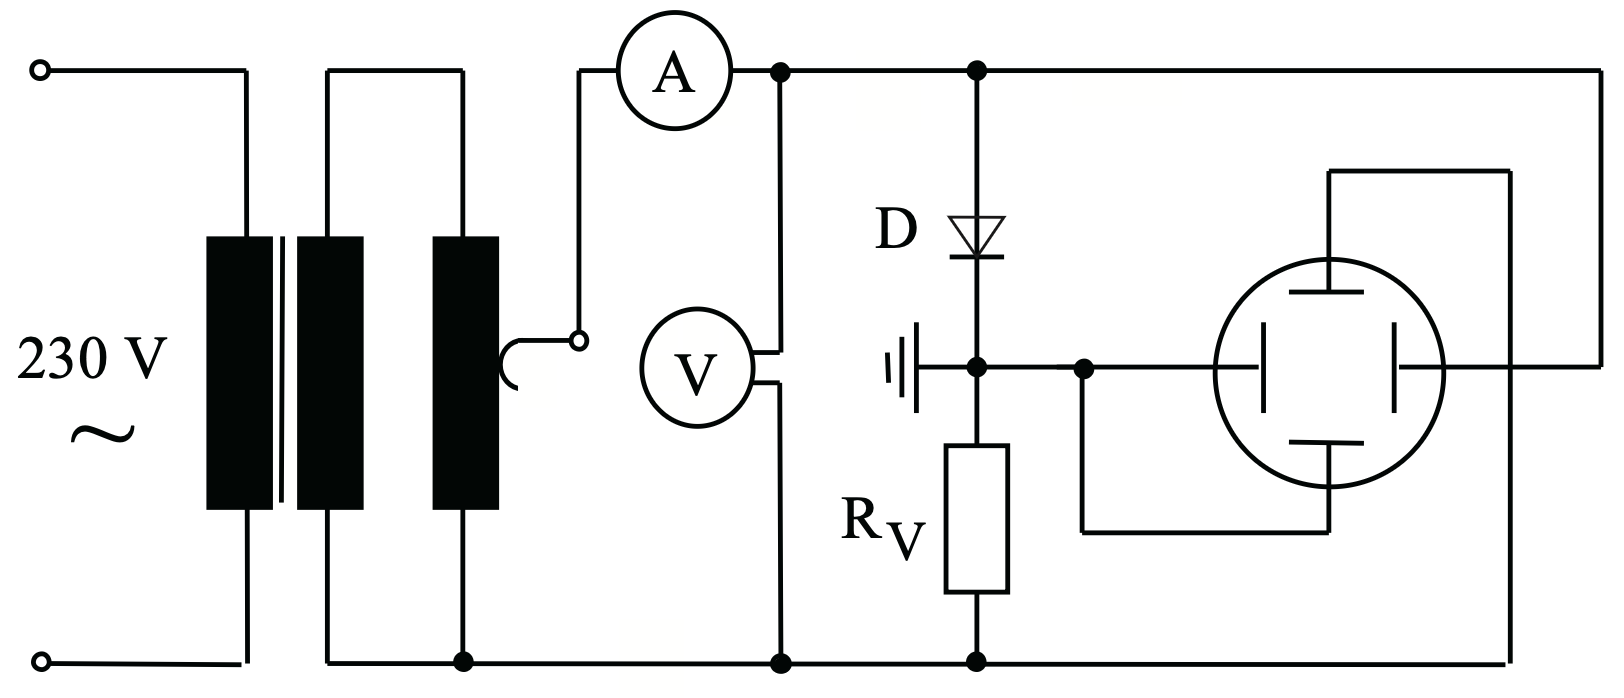
\includegraphics[height=4cm]{images/Schaltung-dioden-kennlinie.png}
		\caption{Abgleich eines Tastkopfes am Oszilloskop mittels Testsignal}\label{fig:schaltung-dioden-kennlinie.png}
	\end{minipage}\hfill
\end{figure}


\marginref{\ref{itm:2-P5-1}}

\marginref{\ref{itm:2-P5-2}}

\marginref{\ref{itm:2-P5-3}}

\marginref{\ref{itm:2-P5-4}}

\marginref{\ref{itm:2-P5-5}}

\subsubsection{Erkenntnisse}

